\lhead[\thepage]{CAPÍTULO \thechapter. PLANIFICACIÓN DEL PROYECTO}
\chead[]{}
\rhead[Patrones de programación paralelos de alto nivel en arquitecturas de memoria distribuida\leftmark]{\thepage}
\renewcommand{\headrulewidth}{0.5pt}

\lfoot[]{}
\cfoot[]{}
\rfoot[]{}
\renewcommand{\footrulewidth}{0pt}

%% This is an example first chapter.  You should put chapter/appendix that you
%% write into a separate file, and add a line \include{yourfilename} to
%% main.tex, where `yourfilename.tex' is the name of the chapter/appendix file.
%% You can process specific files by typing their names in at the 
%% \files=
%% prompt when you run the file main.tex through LaTeX.
\chapter{Planificación del proyecto}
\label{ch:planificacion_proyecto}
\markboth{}{PLANIFICACION DEL PROYECTO}

Este capítulo presenta una planificación detallada del proyecto. Este proyecto ha sido realizado en colaboración con el grupo de investigación \acrshort{arcos} de la Universidad Carlos III de Madrid durante la realización del Máster en Ciencia y Tecnología Informática de la misma universidad. El proyecto comenzó el 8 de enero de 2018 y finalizó el 5 de septiembre de 2018, con un total de 9 meses de trabajo.

Dado que este proyecto de investigación incluye una parte de desarrollo, ambos lados, la investigación y el desarrollo tuvieron que fusionarse para obtener una metodología de investigación y planificación adecuadas. La metodología aplicada se muestra en la Figura\ref{fig:methodology}.

\vspace{0.35cm}
\begin{figure}[htbp]
 	\centering
 	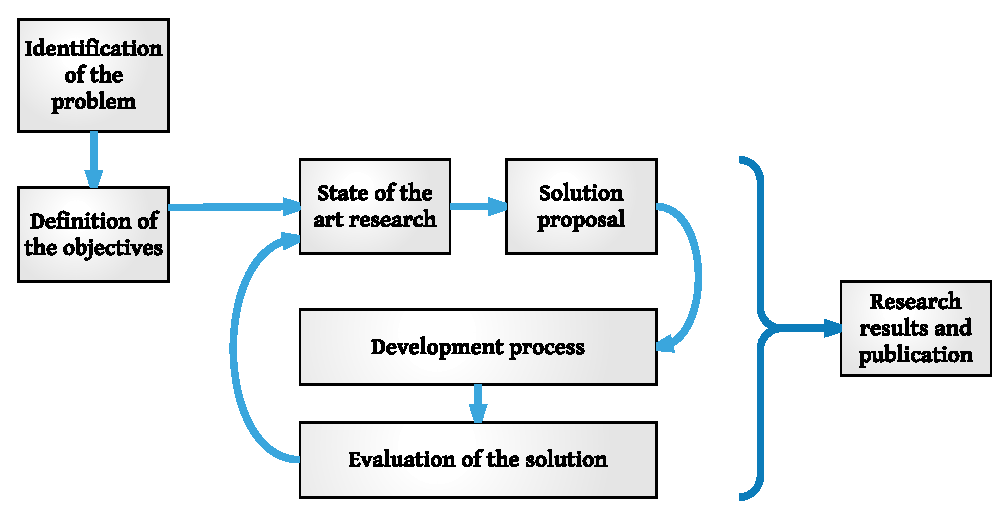
\includegraphics[width=0.75\textwidth]{figures/methodology.pdf}
 	\caption{Metodología de investigación empleada.}
	\label{fig:methodology}
\end{figure}
\vspace{0.35cm}

Donde:

\begin{itemize}

\item \textbf{Identificación del problema} que estamos tratando de resolver.

\item \textbf{Definición de los objetivos} del proyecto.

\item \textbf{Estado de la cuestión a investigar}: sintetiza el más alto nivel del campo científico.

\item \textbf{Propuesta de solución}: diseño y definición de la solución.

\item \textbf{Proceso de desarrollo}: de la solución propuesta.

\item \textbf{Evaluación de la solución}: analizar diferentes casos de estudio.

\item \textbf{Resultados de investigación y publicación}: publica los resultados de la tesis de máster en varias revistas y conferencias.

\item \textbf{Documentación de la tesis}: escribe el informe final.

\end{itemize}

El diagrama de Gantt (Figura \ref{fig:gantt}) muestra todas las tareas realizadas durante el desarrrollo de este trabajo.

\vspace{0.5cm}
\begin{figure}[htbp]
 	\centering
 	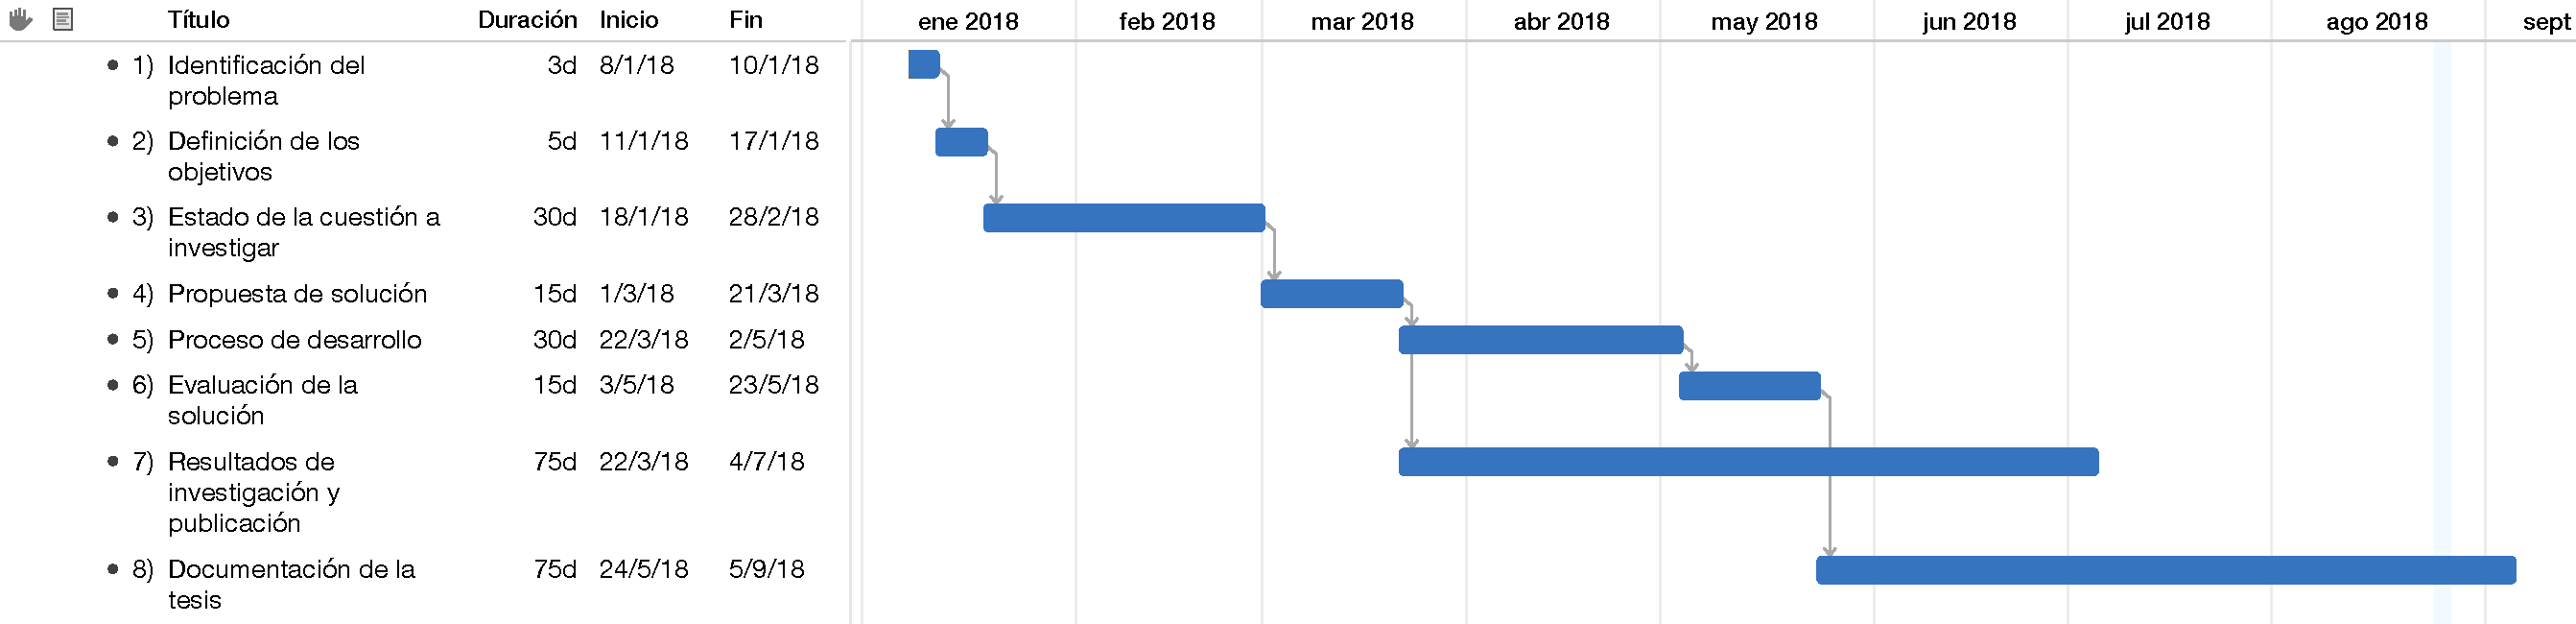
\includegraphics[width=16.5cm]{figures/DiagramaJavi.pdf}
 	\caption{Diagrama de Gantt.}
	\label{fig:gantt}
\end{figure}
\vspace{0.35cm}

%\afterpage{\blankpage} % blank page

